\chapter{METODOLOGÍA DE LA INVESTIGACIÓN}
\section{Diseño de la investigación}
El diseño del presente trabajo de investigación es de tipo experimental puro, ya que se analizarán las variables, procesando los valores con técnicas de regresión para obtener un vector característico que sirva como entrada al modelo de Aprendizaje Profundo, específicamente un modelo de Redes Neuronales Profundas basadas en Grafos.
%Para finalizar se explicará el
%proceso de aplicación de las redes neuronales convolucionales.
\subsection{Tipo de investigación}
El tipo de investigación del presente trabajo es de alcance experimental, ya que el desarrollo de un algoritmo de Aprendizaje Profundo para la detección de rutas seguras en la ciudad de Los Ángeles busca una explicación a partir de patrones que predigan qué rutas son las más seguras basándose en los datos de geolocalización de incidentes delictivos; para ello, se establece una relación de causa efecto, donde a través de una función de riesgo determine qué rutas debe evitar para determinar la opción más segura.


\subsection{Enfoque de investigación}
El enfoque que presenta este trabajo es cuantitativo, ya que utiliza instrumentos de identificación y medición de riesgo en los datos de incidencias, cuyo resultado numérico servirá para entrenar al modelo de Aprendizaje Profundo para detectar qué rutas debe evitar.
\medskip

\section{Población y muestra}
\medskip
\begin{table}[h!]
	\centering
	\begin{tabular}{|m{4cm}|m{10cm}|}
		\hline
		\textbf{Categoría} & \textbf{Descripción} \\
		\hline
		\textbf{Población} & Registro de crímenes extraídos de la página oficial del Departamento de Policía de Los Ángeles, Estados Unidos, desde el año 2020 hasta el año 2024. \\
		\hline
		\textbf{Muestra} & Aproximadamente más de 680,000 registros de crímenes de la página oficial del Departamento de Policía de Los Ángeles. Para la selección de la muestra, se utilizó muestreo no probabilístico o dirigido, ya que se seleccionaron los registros que tienen como descripción aquellos crímenes perpetuados en las calles, tiendas o bancos; como por ejemplo asaltos a mano armada, violación, robo de vehículos, acoso sexual, vandalismo, entre otros. \\
		\hline
		\textbf{Unidad de análisis} & Latitud y Longitud donde ocurrió el crimen registrado. \\
		\hline
		\textbf{Variable y tipo de análisis} & Variable cuantitativa discreta, ya que el presente trabajo se centra en variables numéricas y la medición de riesgo de las rutas. \\
		\hline
	\end{tabular}
\end{table}
\medskip

\section{Operacionalización de Variables}
\medskip
\begin{table}[h!]
	\centering
	\small
	\begin{tabularx}{\textwidth}{|X|X|X|}
		\hline
		\multicolumn{3}{|c|}{\textbf{DEFINICIÓN DE VARIABLES}} \\
		\hline
		\textbf{VARIABLE Y DEFINICIÓN} & \textbf{INDICADOR} & \textbf{FÓRMULA} \\
		\hline
		RUTAS SEGURAS\newline Trayecto el cual evita las zonas con alto nivel de delincuencia para una persona. & Indicador de Riesgo & $R = \sum _{i=1}^{n}(W_{i}\times C_{i})$\newline Donde: 
		\begin{itemize}
			\item $n$ es el número de factores considerados.
			\item $W_{i}$ son los pesos asignados a cada factor.
			\item $C_{i}$ son los valores normalizados de cada factor.
		\end{itemize} \\
		\hline
		\multirow{3}{\hsize}{ALGORITMO DE APRENDIZAJE PROFUNDO\newline Tipo de algoritmo de la subcategoría del Aprendizaje Automático, el cual es el Aprendizaje Profundo, que utiliza Redes Neuronales Artificiales con múltiples capas para el procesamiento y análisis de datos complejos.} & Indicador de Eficiencia & $TTM = N_{ep} \times T_{ep}$ \newline Donde: 
		\begin{itemize}
			\item $N_{ep}$ es el número de épocas del modelo.
			\item $T_{ep}$ el tiempo promedio necesario para completar una época en el entrenamiento.
		\end{itemize}\\
		\cline{2-3}
		& Indicador de Precisión & $RMSE = \sqrt{\frac{1}{n}\sum _{i = 1}^{n}(y_{i}-\hat{y}_{i})^{2}}$ \newline Donde: 
		\begin{itemize}
			\item $n$ es el número total de observaciones o datos.
			\item $y_{i}$ es el valor observado en la posición $i$.
			\item $\hat{y}_{i}$ es el valor predicho en la posición $i$.
		\end{itemize}\\
		\cline{2-3}
		& Tasa de éxito del agente & $Success\: Rate = \frac{Number\,of \, Successful\,Routes}{Total\,Number\,of \, Routes}$ \\
		\hline
	\end{tabularx}
\end{table}
\medskip
\section{Técnicas de recolección de datos}
Para el presente trabajo se recolectó un conjunto de datos de registros públicos de crímenes en la ciudad de Los Ángeles, que se componen de variables tanto cuantitativas (longitud, latitud, fecha, área, número de documento, edad, entre otros), como cualitativas (descripción del crimen, dirección, sexo, entre otros). Para obtener este conjunto de datos se siguió un flujo de búsqueda, descarga y segmentación de los registros de crímenes en base al tipo de crimen realizado como se muestra en la figura. Cabe mencionar que en proceso de segmentación, el conjunto de datos contiene una columna llamada “Crm Cd Desc”, que son los tipos de crímenes registrados, por lo que se filtra aquellos crímenes que involucren agresión física o verbal, como también vandalismos en las zonas urbanas de una ciudad. Asimismo, se extraerá en formato XLSX solo las columnas necesarias para el entrenamiento del modelo, los cuáles son: Crm Cd Desc, Date Rptd, LAT, LON. “LAT” y “LON” representan la latitud y longitud donde ocurrió el crimen.
\medskip
\begin{figure}[h]
	\begin{center}
		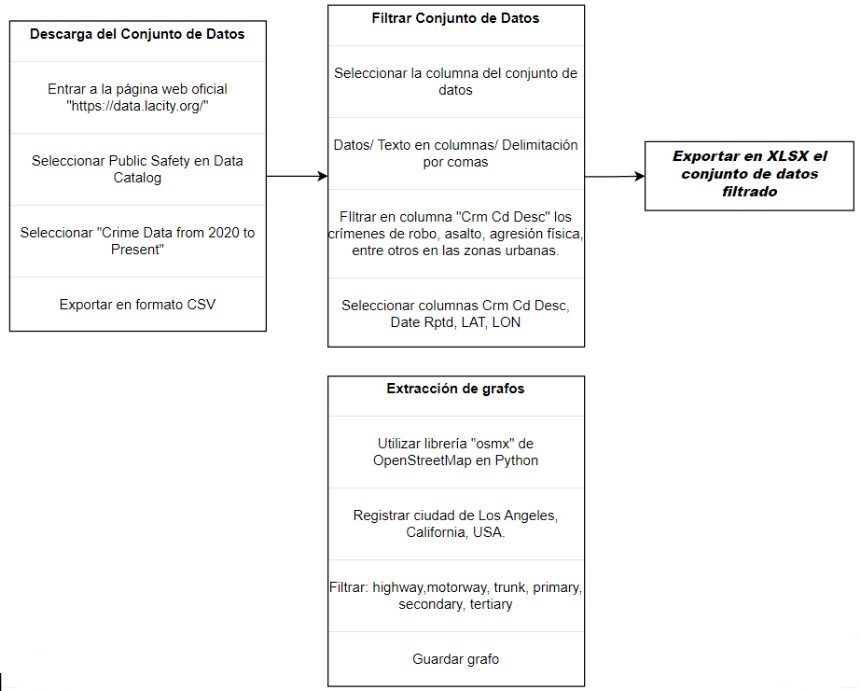
\includegraphics[width=0.7\textwidth]{3/figures/flujoreco.jpg}
		\caption[Elaboración propia: Flujo de recolección de datos]{Elaboración propia: Flujo de recolección de datos}
		\label{1:fig}
	\end{center}
\end{figure}
\medskip
Además de la extracción del conjunto de datos de registro de crímenes, es importante extraer la cartografía de la ciudad de Los Ángeles, como se muestra en la figura, haremos uso de la librería “osmnx” de OpenStreetMaps en Python para extraer los datos de una zona que buscas según lo que necesitas. Para el presente trabajo, se busca la región de la ciudad de Los Ángeles, el cual la librería nos brindará todas los nodos que son las calles, estaciones, avenidas, entre otros.

\section{Técnicas para el procesamiento y análisis de la información}
Para la metodología propuesta, se usó de base la metodología CRISP-DM(Cross-Industry Standard Process for Data Mining), que está orientado mayormente al campo de la minería de datos, es un proceso o un ciclo de vida del desarrollo de un modelo, y el cuál es altamente personalizable y flexible en cualquier tipo de situación o desarrollo \parencite{gl_crisp}. Este ciclo de vida del modelo consta de 6 fases, las cuales son:

%\begin{enumerate}
%	\item Like this,
%	\item and like this.
%\end{enumerate}
\begin{itemize}
	\item Entendimiento del modelo: La comprensión de los objetivos y requisitos definidos del proyecto para el usuario final, con el fin de convertir dicho conocimiento en una definición técnica del problema.
	\item Comprensión de los datos: Se realiza un análisis exploratorio en los datos para tener una visión general de lo que se puede conseguir de estas.
	\item Preparación de los datos: En esta fase se cubre todas las actividades requeridas para la construcción del conjunto de datos, junto con el preprocesamiento de los datos que serán empleados para la siguiente fase.
	\item Modelado de datos: Fase el cuál tiene que ver con la implementación de los modelos requeridos del proyecto que derivarán a los próximos resultados y conclusiones de este.
	\item Evaluación: Se mide los resultados y calidad del modelo, junto con su efectividad para el cumplimiento de los requisitos establecidos.
	\item La implementación del modelo en un entorno operativo, la planificación del mantenimiento y monitoreo de este para que siga cumpliendo con los objetivos del proyecto.
\end{itemize}
Estableciendo la base teórica en lo que consiste la metodología CRISP-DM, también se usó de ejemplo la metodología propuesta por \citeauthor{pr_saferoute} en su artículo \citetitle{pr_saferoute}, ya que estos trabajan también con conjuntos de datos de delitos y la obtención del mapa de las ciudades en OpenStreetMaps, además que implementa una función de recompensa basada en riesgos para entrenar su modelo de Aprendizaje por Refuerzo. Otro artículo de inspiración para el desarrollo de la metodología, es de \citeauthor{pr_esquivel} en su artículo \citetitle{pr_esquivel}, ya que proponen la aplicación de regresión LOESS para el preprocesamiento de los datos que serán utilizadas para el entrenamiento de su modelo LSTM basado en grafos. Por último, también tomará de guía el flujo de condición para la elección de rutas seguras propuesta por \citeauthor{pr_Soni} en su artículo \citetitle{pr_Soni}. La metodología del presente trabajo de investigación se puede visualizar de manera gráfica en la Figura \ref{1:mark}.\medskip

\begin{figure}[h]
	\begin{center}
		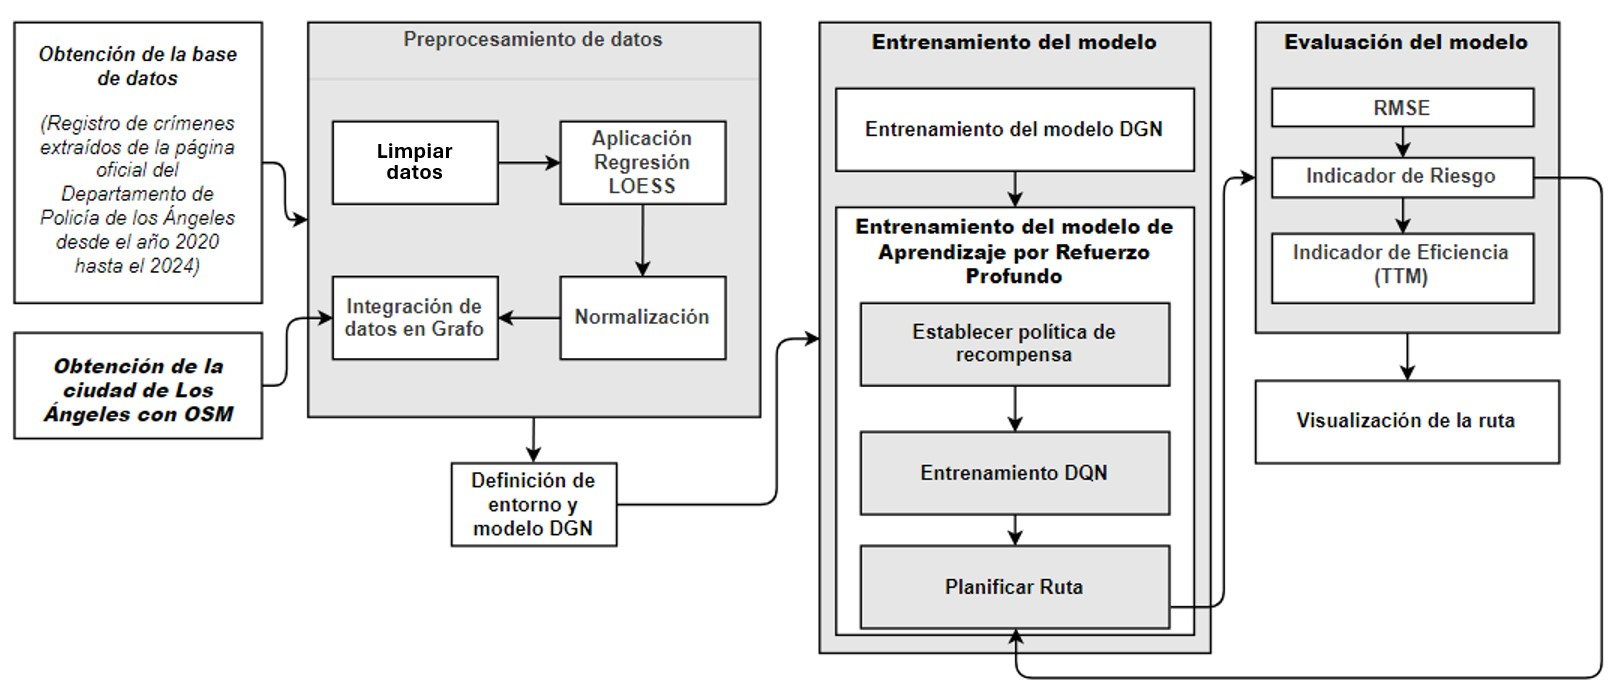
\includegraphics[width=0.7\textwidth]{3/figures/metopropuesta.jpg}
		\caption[Elaboración propia: Metodología propuesta]{Elaboración propia: metodología propuesta}
		\label{1:mark}
	\end{center}
\end{figure}
\medskip
Como ya se mencionó, esta metodología viene de la derivación de la metodología tradicional CRISP-DM junto con las metodologías propuestas en los antecedentes. Se puede encontrar una relación entre la comprensión del negocio con el objetivo del presente artículo el cuál es la minimización del riesgo en la detección de rutas seguras. Asimismo, en la fase de la comprensión de los datos, se encuentra la recolección de los registros de crímenes en la ciudad de Los Ángeles y la obtención de la ciudad de Los Ángeles en OpenStreetMap. La fase de preparación de los datos es más que la fase del preprocesamiento de los datos con sus respectivos pasos propuestos por la metodología. Mientras que el Modelado es la creación y entrenamiento del modelo de Deep Graph Network (DGN) para la representación del grafo de la ciudad y del entrenamiento del modelo de Aprendizaje por Refuerzo Profundo para establecimiento de las políticas de recompensa y la planificación y detección de rutas seguras. Por último, las fases de evaluación y despliegues son las métricas propuestas en la metodología que determinará qué ruta segura debe elegir el usuario según el índice de riesgo que presente.
\subsection{Metodología de la implementación de la solución}
\subsubsection{Adquisición}
En esta fase se describe la obtención del conjunto de datos, como ya se mencionó anteriormente en el punto de las técnicas de recolección, se necesita registros de crímenes realizados en una zona urbana, para esto, se decidió trabajar con el conjunto de datos abiertos de registros de crimen en la ciudad de Los Ángeles desde el 2020 hasta el 2024. Dicho conjunto de datos tiene más de novecientos veinticinco mil registros aproximadamente y cuenta con 28 columnas las cuáles se detallan a continuación:


\begin{longtable}{|p{2.5cm}|p{6cm}|p{5cm}|}
	\hline
	\textbf{Nombre de Columna} & \textbf{Descripción} & \textbf{Tipo de dato} \\
	\hline
	\endfirsthead
	
	\multicolumn{3}{c}{{\tablename\ \thetable{} -- Continuación de la página anterior}} \\
	\hline
	\textbf{Nombre de Columna} & \textbf{Descripción} & \textbf{Tipo de dato} \\
	\hline
	\endhead
	
	\hline
	\multicolumn{3}{r}{{Continúa en la siguiente página}} \\
	\endfoot
	
	\hline
	\caption{Descripción de las columnas del conjunto de datos de LAPD \\
		Fuente: \citep*{gl_LAPD}. \citetitle{gl_LAPD}.} \label{tab:lapd-data-description} \\
	\endlastfoot
	
	DR\_NO & Número de División de Registros: Número de archivo oficial compuesto por un año de 2 dígitos, un ID de área y 5 dígitos & Texto \\
	\hline
	Date Rptd & MM/DD/YYYY Floating Timestamp & Texto \\
	\hline
	DATE OCC & MM/DD/YYYY Floating Timestamp & Texto \\
	\hline
	TIME OCC & En horario militar de 24 horas & Texto \\
	\hline
	AREA & El LAPD tiene 21 comisarías comunitarias denominadas áreas geográficas dentro del departamento. & Texto \\
	\hline
	AREA NAME & Las 21 áreas geográficas o divisiones de patrulla también reciben una designación de nombre que hace referencia a un punto de referencia o a la comunidad circundante. & Texto \\
	\hline
	Rpt Dist No & Un código de cuatro dígitos que representa una subárea dentro de un Área Geográfica. & Texto \\
	\hline
	Part 1-2 & Sin descripción & Número \\
	\hline
	Crm Cd & Indica el delito cometido. (Igual que el Código Penal 1) & Texto \\
	\hline
	Crm Cd Desc & Define el Código Penal previsto. & Texto \\
	\hline
	Mocodes & Modus Operandi: actividades asociadas con el sospechoso en la comisión del delito. & Texto \\
	\hline
	Vict Age & Numérico de dos caracteres & Texto \\
	\hline
	Vict Sex & F - Mujer M - Hombre X - Desconocido & Texto \\
	\hline
	Vict Descent & Código de ascendencia: A - Otro asiático ... Z - Indio asiático & Texto \\
	\hline
	Premis Cd & El tipo de estructura, vehículo o lugar donde ocurrió el delito. & Número \\
	\hline
	Premis Desc & Define el Código de Premisa proporcionado. & Texto \\
	\hline
	Weapon Used Cd & El tipo de arma utilizada en el delito. & Texto \\
	\hline
	Weapon Desc & Define el código de arma utilizada proporcionado. & Texto \\
	\hline
	Status & Estado del caso. (IC es el valor predeterminado) & Texto \\
	\hline
	Status Desc & Define el código de estado proporcionado. & Texto \\
	\hline
	Crm Cd 1 & Indica el delito cometido. El Código Penal 1 es el principal y el más grave. & Texto \\
	\hline
	Crm Cd 2 & Puede contener un código para un delito adicional, menos grave que el Código Penal 1. & Texto \\
	\hline
	Crm Cd 3 & Puede contener un código para un delito adicional, menos grave que el Código Penal 1. & Texto \\
	\hline
	Crm Cd 4 & Puede contener un código para un delito adicional, menos grave que el Código Penal 1. & Texto \\
	\hline
	LOCATION & Dirección del incidente del crimen redondeada a la centena de cuadra más cercana para mantener el anonimato. & Texto \\
	\hline
	Cross Street & Cruce de Calle de Dirección Redondeada & Texto \\
	\hline
	LAT & Latitud & Número \\
	\hline
	LON & Longitud & Número \\
	\hline
\end{longtable}

Dicho conjunto de datos se seleccionarán las columnas importantes que servirán para el entrenamiento del modelo propuesto, los cuáles son las columnas Crm Cd Desc, Date Rptd, LAT y LON. Con respecto al tipo de crimen, este conjunto de datos contiene múltiples registros que van desde vandalismo callejero a fraude financiero, por lo que se decidió filtrar manualmente en la columna Crm Cd Desc lo siguiente: VEHICLE - STOLEN, BURGLARY FROM VEHICLE, BIKE - STOLEN, SHOPLIFTING-GRAND THEFT (\$950.01 \& OVER), BATTERY - SIMPLE ASSAULT, CRM AGNST CHLD (13 OR UNDER) (14-15 \& SUSP 10 YRS OLDER), ASSAULT WITH DEADLY WEAPON, AGGRAVATED ASSAULT,	CRIMINAL THREATS - NO WEAPON DISPLAYED, THEFT FROM MOTOR VEHICLE - PETTY (\$950 \& UNDER)	BURGLARY, THEFT PLAIN - PETTY (\$950 \& UNDER), THEFT FROM MOTOR VEHICLE - GRAND (\$950.01 AND OVER), ROBBERY, BUNCO, GRAND THEFT, BATTERY WITH SEXUAL CONTACT, SHOPLIFTING - PETTY THEFT (\$950 \& UNDER), VANDALISM - FELONY (\$400 \& OVER, ALL CHURCH VANDALISMS), RAPE, FORCIBLE, VANDALISM - MISDEAMEANOR (\$399 OR UNDER), OTHER ASSAULT, PICKPOCKET, DISTURBING THE PEACE, BUNCO, ATTEMPT, PEEPING TOM, ATTEMPTED ROBBERY, CHILD STEALING, INDECENT EXPOSURE, STALKING, BURGLARY, ATTEMPTED, RAPE, ATTEMPTED, DISCHARGE FIREARMS/SHOTS FIRED, VEHICLE - ATTEMPT STOLEN, BURGLARY FROM VEHICLE, ATTEMPTED	THEFT, PERSON, VEHICLE, STOLEN - OTHER (MOTORIZED SCOOTERS, BIKES, ETC), THEFT FROM PERSON - ATTEMPT, BOMB SCARE, ASSAULT WITH DEADLY WEAPON ON POLICE OFFICER, SHOTS FIRED AT INHABITED DWELLING	KIDNAPPING - GRAND ATTEMPT, SHOTS FIRED AT MOVING VEHICLE, TRAIN OR AIRCRAFT, THROWING OBJECT AT MOVING VEHICLE	KIDNAPPING, CRIMINAL HOMICIDE, PURSE SNATCHING, THEFT FROM MOTOR VEHICLE - ATTEMPT, SHOPLIFTING - ATTEMPT, PROWLER, MANSLAUGHTER, NEGLIGENT, PURSE SNATCHING - ATTEMPT, BIKE - ATTEMPTED STOLEN, PICKPOCKET, ATTEMPT.

Todos los tipos de crímenes mencionados están relacionados con robos, asaltos, vandalismo, agresión física o sexual en las zonas públicas, asalto a pequeñas tiendas, acoso, intento de robo, entre otros. La principal razón por la que se debe filtrar este tipo de crímenes es para que el modelo pueda predecir las rutas seguras en base a crímenes perpetrados en las calles. Esto da más de seiscientos mil registros.

\textbf{Entregable:} Conjunto de datos con columnas requeridas para el entrenamiento del modelo filtrado por crímenes ocasionados en las calles de la ciudad.

Además de la adquisición del conjunto de datos, se debe obtener el mapa de la zona de la ciudad de Los Ángeles, con el fin de tener las calles, avenidas, estaciones y vías que servirá al modelo para la creación del grafo. Para esto se hará uso de la librería de OpenStreetMap llamada “OSMX” y qué en base a una consulta realizada en Python filtrado con los parámetros "highway", "motorway”, “trunk”, “primary”, “secondary”, “tertiary" , se obtendrá los nodos y vértices de la ciudad.

\textbf{Entregable:} Grafo de las calles de la ciudad de Los Ángeles obtenidos de la librería OSMX.
\medskip

\begin{figure}[h]
	\begin{center}
		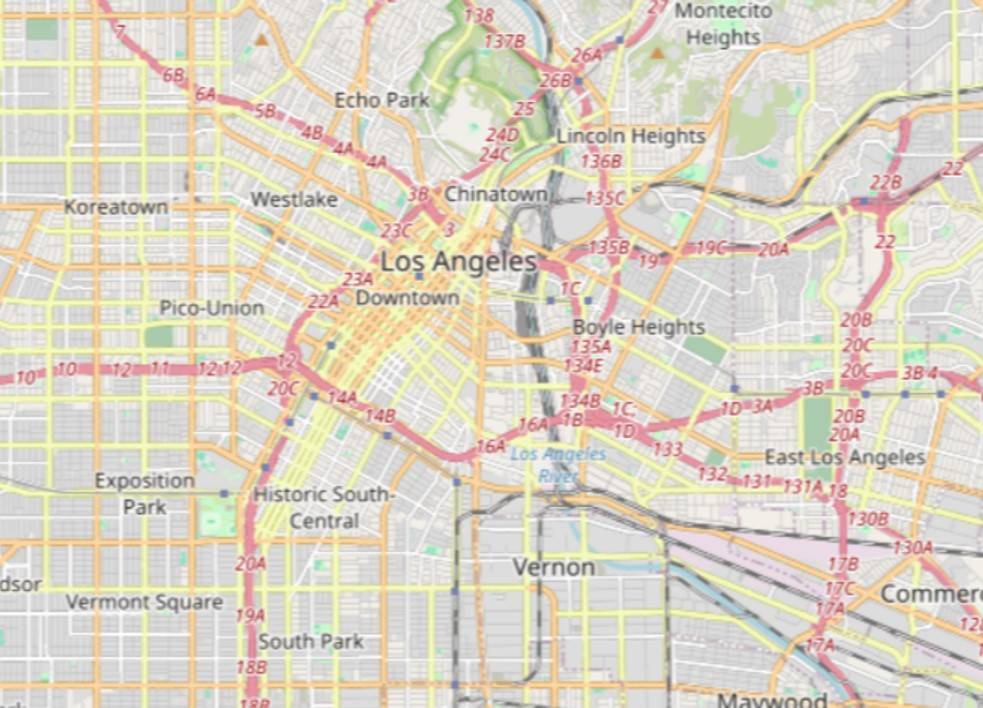
\includegraphics[width=0.65\textwidth]{3/figures/grafoa.jpg}
		\caption[Zona de la ciudad de Los Ángeles en OpenStreetMap]{Zona de la ciudad de Los Ángeles en OpenStreetMap}
		\label{1:fig}
	\end{center}
\end{figure}
\medskip

\subsubsection{Preprocesamiento de datos}

En esta fase se realizará 4 pasos para que la carga de la información esté lista y limpia para hacer su uso en la etapa de entrenamiento del modelo, por lo que se detallará a continuación los siguientes pasos.

\begin{itemize}
	\item[a.] Limpieza de dato \\

Este primer paso ayudará en primera instancia a eliminar los datos vacíos que se encuentran en la base de datos de registro de crímenes. Esto puede causar problemas a la hora de entrenar el modelo y reducir la precisión de este, por lo que es esencial mantener la integridad del conjunto de datos, para esto, Python cuenta con múltiples librerías o lista de comandos que le permite eliminar los datos faltante según los parámetros que se le imponga, una de las más conocidas es “.dropna()”.

El segundo paso el cambio de tipo de variable, ya que el conjunto de datos está compuesto mayoritariamente por variables de tipo texto que no deberían ser consideradas de esa manera, hacer un correcto cambio en el tipo de variables permitirá hacer un análisis de series de tiempo más eficiente y preciso o aplicarla correctamente en los pasos posteriores como la aplicación de regresión LOESS.  Python también ofrece múltiples listas de comandos que permiten cambiar el tipo de variable según las necesidades requeridas del proyecto.

\textbf{Entregable:} Conjunto de datos completo con la correcta clasificación de sus variables.
	\item[b.] Aplicación Regresión LOESS \\
	
La Regresión LOESS	es un método que combina la regresión lineal con la regresión no lineal, ajustando modelos sencillos sobre subconjuntos locales de datos para la creación de una función que describa la variación de los datos. En cada punto del conjunto de datos se ajusta una regresión polinómica dando más peso a los puntos cercanos y menos peso a los más lejanos, esto puede ayudar para la determinar la relación entre entre las variables y sobre todo, el manejo de datos ruidosos, es decir, si presenta una gran variabilidad en los datos, por lo que puede resaltar las tendencias para entender mejor las áreas donde hay más crímenes, proporcionando una visión más clara de los patrones de los datos y mejorando la identificación de zonas de alto riesgo \parencite{gl_maxima}.

Para esto, se selecciona primero cada punto de interés Xi, para la asignación de pesos se utiliza la siguiente fórmula:

\begin{equation} 
	w_{i}(x)=(1-\begin{vmatrix}
		\frac{x-x_{i}}{d_{max}}
	\end{vmatrix}^{3})^{3}
\end{equation}

Donde $d_{max}$ es la distancia máxima dentro del vecindario.
Adicionalmente a esto, se realiza el ajuste del Polinomio local en término de matrices, el cual se hace minimizando la suma ponderada de los errores cuadrado:

\begin{equation} 
	\sum_{i}w_{i}(x)(y_{i}-(\beta _{0}+\beta _{1}(x_{i}-x)))^{2}
\end{equation}

Donde $y_{i}$ son los valores de respuesta.

\textbf{Entregable:} Conjunto de datos suavizados de los crímenes con baja variabilidad de estos.

	\item[c.] Normalización \\

Dado a que se trabaja con la latitud y longitud, es importante el proceso de la normalización para que tengan una escala similar, esto ayuda a mejorar la eficiencia y precisión del modelo. Se hará uso de la normalización Min-Max, ya que asegura que todos los atributos están el el rango de 0 a 1, asimismo ayuda a preservar las relaciones entre los valores originales y es compatible con muchos algoritmos\parencite{gl_med}. 
	\begin{equation} 
		{x}'=\frac{x-x_{min}}{x_{max}-x_{min}}
	\end{equation}

Donde:

$x$ es el valor original.

$x_{min}$ es el valor mínimo de la característica.

$x_{max}$ es el valor máximo de la característica.

${x}'$ es el valor normalizado.

\textbf{Entregable:} Conjunto de datos normalizados en un mismo rango.
	
	\item[d.] Normalización \\
	
Este paso es necesario para el análisis y toma de decisiones del modelo, por lo que se debe contar con la estructura geográfica de la ciudad representada en grafo de OpenStreetMap, junto con el conjunto de datos ya normalizados. Para la evaluación del riesgo de una ruta, se debe asociar cada registro de crimen con el vértice más cercano (intersección) o con la arista (calle) dónde ocurrió en la ciudad, para esto se utiliza la distancia euclidiana, el cual se representa de la siguiente manera:

\begin{equation} 
	d=\sqrt{(x_{2}-x_{1})^{2}+(y_{2}-y_{1})^{2}}
\end{equation}

Dónde $(x_{1},y_{1})$ son las coordenadas del crimen y $(x_{2},y_{2})$ son las coordenadas del vértice del grafo.

\textbf{Entregable:} Conjunto de datos integrado en el grafo de la ciudad para su uso en la fase de entrenamiento.

\end{itemize}

\subsubsection{Definición de entorno y modelo DGN}

La definición de un entorno para el entrenamiento del modelo es fundamental para proporcionar una plataforma robusta y flexible para encontrar rutas seguras en el grafo de la ciudad, para esto se hará uso del entorno Gym, que es un paquete proporcionado por Python y que da la facilidad de establecer reglas y la capacidad de interactuar con el entorno del grafo de la ciudad para la toma de decisiones y recibir recompensas basadas en el riesgo \parencite{gl_gym}. Asimismo, Gym puede facilitar la implementación de algoritmos DGN y diferentes algoritmos DRL, además de ser compatibles con diversas bibliotecas de Aprendizaje Profundo como TensorFLow, Pytorch, entre otros que facilita la integración de los algoritmos de DRL como DQN.
Para la elección de un modelo DGN, se optó por utilizar el modelo Graph Convolutional Network (GCN), por su capacidad de modelar relaciones complejas entre los nodos y aristas en grafos para saber cómo están distribuidos los crímenes a lo largo de las calles y vecindarios. Asimismo, GCN tiene la capacidad de procesar eficientemente datos espaciales en el grafo que le permite integrar los datos de los registros de crímenes ya que se manejan según coordenadas. Debido a que la ciudad de Los Ángeles está compuesta por muchas calles y avenidas que se interceptan entre sí, esto hace que sea un grafo grande y complejo, el cual un modelo GCN es flexible y adaptable a ese sin necesidad de establecer características específicas \parencite{gl_git}.
\medskip

\begin{figure}[h]
	\begin{center}
		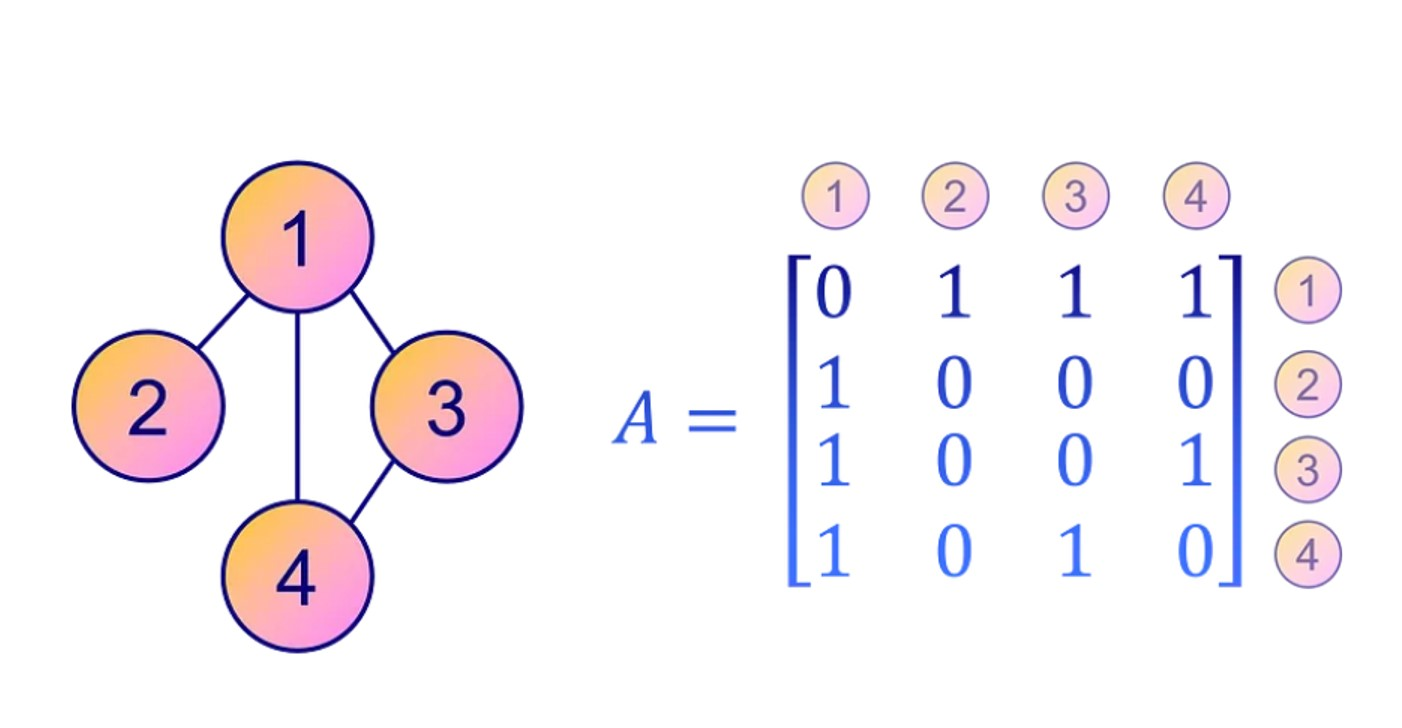
\includegraphics[width=0.65\textwidth]{3/figures/grafosim.jpg}
		\caption[Estructura simple de un grafo]{Estructura simple de un grafo\\
			Fuente: \citep*{gl_gnnmed}. \citetitle{gl_gnnmed}.}
		\label{1:fig}
	\end{center}
\end{figure}
\medskip
\textbf{Entregable:} Entorno de trabajo en Gym utilizando el modelo GCN para la fase del entrenamiento.

\subsubsection{Entrenamiento del Modelo}

Para el entrenamiento del modelo DGN, este será realizado en el entorno de TensorFlow, el cual permite la construcción de modelos de Aprendizaje Profundo complejos y personalizados, definiendo capas personalizadas, funciones de activación y de pérdida. Otra de las razones es porque está optimizado para realizar cálculos en grandes volúmenes de datos y que está respaldado por Google y una gran comunidad de desarrolladores, brindándonos abundante contenido y documentación para la implementación efectiva del GCN
\begin{itemize}
	\item[a.] Entrenamiento del modelo DGN \\
	
Para el entrenamiento del modelo DGN, este será realizado en el entorno de TensorFlow, el cual permite la construcción de modelos de Aprendizaje Profundo complejos y personalizados, definiendo capas personalizadas, funciones de activación y de pérdida. Otra de las razones es porque está optimizado para realizar cálculos en grandes volúmenes de datos y que está respaldado por Google y una gran comunidad de desarrolladores, brindándonos abundante contenido y documentación para la implementación efectiva del GCN.
\medskip

\begin{figure}[h]
	\begin{center}
		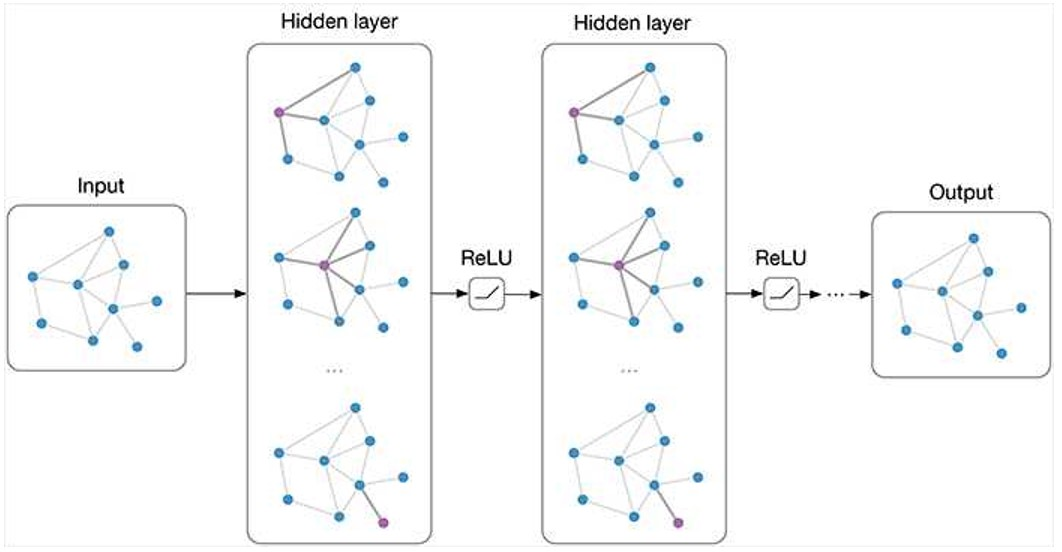
\includegraphics[width=0.65\textwidth]{3/figures/estru.jpg}
		\caption[Estructura de GCN]{Estructura de GCN\\
			Fuente: \citep*{gl_aisummer}. \citetitle{gl_aisummer}.}
		\label{1:fig}
	\end{center}
\end{figure}
\medskip

En cuanto a las funciones de activación, se utilizará la función de activación ReLU (Rectified Linear Unit), ya que el modelo GCN requiere de funciones de activación no lineales para aprender y modelar las relaciones complejas entre los datos y mejora el rendimiento del modelo teniendo una mejor capacidad de identificar zonas de alto riesgo de crimen. Esta función de activación es representada matemáticamente como:

\begin{equation} 
	ReLU=max(0,x)
\end{equation}

Donde $x$ es un valor de entrada, y que la función devuelve 0 si en caso $x$ es negativo y si es positivo devuelve $x$.

Está función de activación ReLU será empleada en cada capa oculta del modelo.

En cuanto a la función de activación de la capa de salida, se utilizará la función Sigmoid, el cuál comprime los valores de entrada a un rango entre 0 y 1, útil para predecir la probabilidad de riesgo de crímen para cada nodo del grafo y que de esta manera el agente pueda determinar qué ruta tomar en modelo DRL. La función de activación es representada matemáticamente de la siguiente manera:

\begin{equation} 
	Sigmoid(x)=\frac{1}{1+e^{-x}}
\end{equation}

Se emplea la fórmula de propagación el cual permite actualizar las características de cada nodo en función de las características de sus vecinos, con el fin de capturar relaciones estructurales en el grafo, este aprenderá los pesos con el fin de minimizar la función de pérdida, ajustando para mejorar la predicción del riesgo. Esta fórmula es representada de la siguiente manera:

\begin{equation} 
	h_{v}^{l+1}=\sigma (\sum_{u \in  N(v)}\frac{1}{c_{uv}}h_{v}^{l}W^{l})
\end{equation}

Donde:

$h_{v}^{l}$ es la representación del nodo $v$ en la capa $l$.

$N(v)$ son los nodos vecinos de $v$.

$c_{uv}$ es el factor de la normalización de la arista entre $u$ y $v$.

$W^{l}$ es la matriz de pesos en la capa $l$.

$\sigma$ es la función de activación.

Por último se emplea un optimizador para el entrenamiento del modelo en TensorFlor, siendo el más conocido el Optimizador Adam (Adaptive Moment Estimation), que funciona en diversos problemas, ajustando automáticamente la tasa de aprendizaje en función se su estimación del momento \parencite{gl_interactive}.

\textbf{Entregable:} Representaciones de las características de riesgo de crimen en un grafo para el entrenamiento del modelo DRL y la probabilidad de riesgo de cada nodo.

\item[b.] Entrenamiento del modelo de Aprendizaje por Refuerzo Profundo \\
\begin{itemize}
	\item Establecer política de recompensa \\

Para el establecimiento de una política de recompensa, la cuál le servirá al agente determinar qué ruta será la más segura, se hará uso de las probabilidades de riesgo de cada nodo obtenidas en el entrenamiento del modelo DGN, además de establecer un umbral, que es de 0.6 y que representa el valor máximo que puede tomar el agente para elegir qué ruta tomar. Para esto, se propone la siguiente fórmula:

\begin{equation} 
	Recompensa = \left\{\begin{matrix}
		R_{safe}\; \; \; si\; Indice \;de\;Riesgo\;\leq \theta \\ 
		R_{risk}\; \; \; si\; Indice \;de\;Riesgo\;>  \theta 
	\end{matrix}\right.
\end{equation}

En cada nodo que el agente visite, este determinará mediante la función de recompensa si debe tomar dicho nodo, si en caso el índice de riesgo es menor al umbral, lo selecciona, caso contrario, lo evita.

\textbf{Entregable:} Función de recompensa para el entrenamiento del modelo DQN.

	\item Entrenamiento DQN \\

Para que el modelo aprenda a elegir la ruta más segura basándose en la política de recompensa ya establecida anteriormente, se decide entrenar un agente en un modelo DQN, ya que tiene la capacidad de manejar problemas de toma de decisiones mediante la interacción en entornos complejos y de alta dimensionalidad como lo es el grafo de la ciudad de Los Ángeles. Para el correcto entrenamiento del modelo DQN, se debe considerar los siguientes parámetros:
\begin{itemize}
	\item \textbf{Replay Buffer Size:} Este parámetro tiene como propósito el de almacenar las experiencias del agente, es decir, es una memoria que incluye el estado, la acción tomada, la recompensa recibida y el siguiente estado resultando, haciendo que el entrenamiento sea más estable y eficiente \parencite{gl_ray}. El tamaño que se define comúnmente es de 100,000 experiencias. Sin embargo, el establecimiento del tamaño de experiencia depende de la memoria y tiempo de muestreo durante el entrenamiento.
	\item \textbf{Minibatch Size:} Número de experiencias muestreadas del parámetro anterior de cada red neuronal y ayuda a estabilizar el aprendizaje con un correcto uso de los recursos computacionales. Los valores típicos son 32 o 64.
	\item \textbf{Learning rate:}  Es la tasa de aprendizaje del modelo y el encargado de ajustar o controlar el tamaño de los pesos de la red neuronal. El valor comúnmente utilizado es 0.001. Se debe evitar utilizar una tasa de aprendizaje mayor ya que puede volver inestable el modelo, asimismo, si la tasa es muy baja puede aumentar el tiempo de aprendizaje del modelo DRL \parencite{gl_findin}.
	\medskip
\begin{figure}[h]
	\begin{center}
		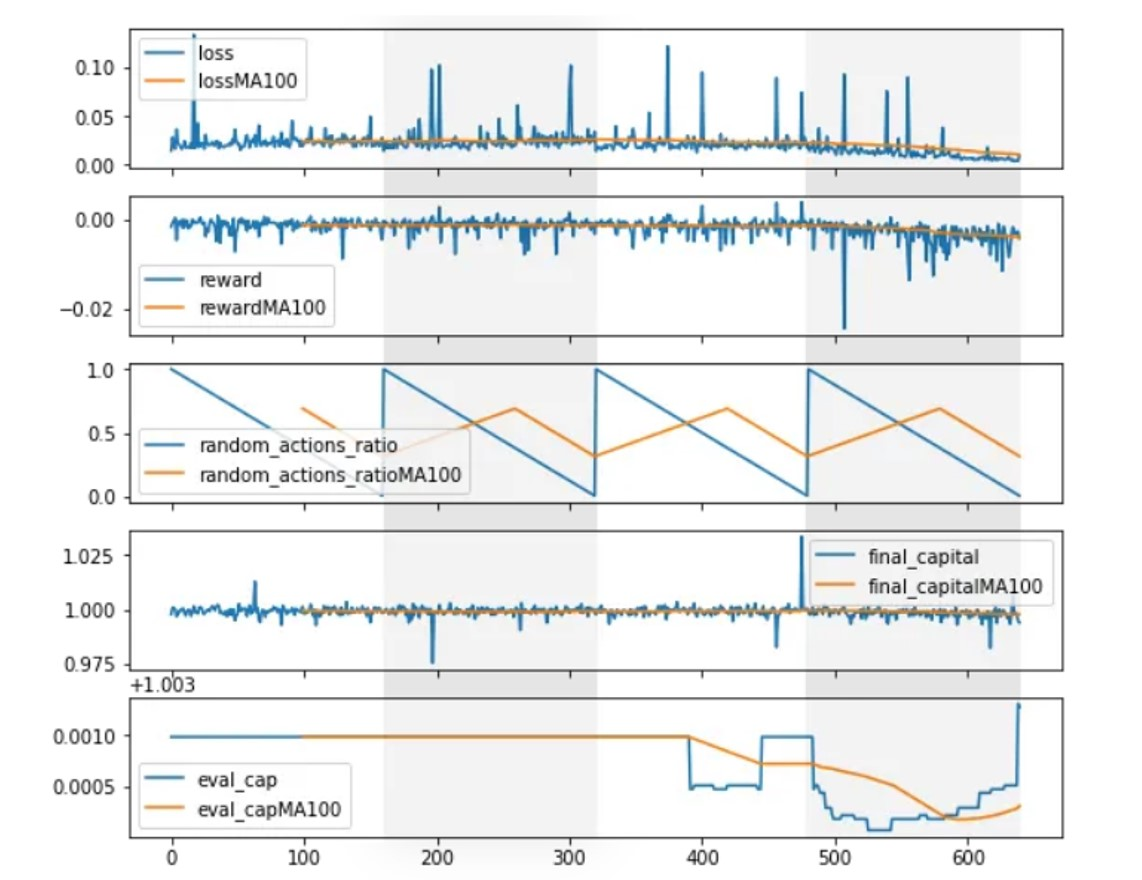
\includegraphics[width=0.65\textwidth]{3/figures/learning.jpg}
		\caption[Experimentación de tasa de aprendizajes]{Experimentación de tasa de aprendizajes\\
			Fuente: \citep*{gl_findin}. \citetitle{gl_findin}.}
		\label{1:fig}
	\end{center}
\end{figure}
\medskip
	
	\item \textbf{Discount Factor:} Determina la importancia de las recompensas, controlando la valoración que le asigna el agente a la recompensa frente a las recompensas futuras. El valor de recompensa varía de 0 a 1, siendo los valores típicos entre 0.9 y 0.99; este valor determina que tan importante es para el agente las recompensas futuras, por lo que sí es bajo, valorará más las recompensas inmediatas. Esto puede ayudar al modelo de detección de rutas seguras para saber si vale la pena seguir al siguiente nodo.
	\item \textbf{Exploration Rate:} Es un parámetro que controla la probabilidad de que el agente tome una acción, esto facilita el equilibrio entre la política aprendida y la exploración de nuevas acciones. Este paso es importante para el modelo, porque le permitirá explorar más las diversas calles de la ciudad, que serían los nodos, para que el agente descubra nuevas estrategias. Usualmente se inicia con un valor alto de 1 en exploración y mediante se va entrenando el modelo va disminuyendo gradualmente.
	
	\item \textbf{Target Network Update Frequency:} Es la frecuencia con la que se actualiza la red con el fin de estabilizar el entrenamiento con número de pasos establecidos. Se debe seleccionar la cantidad de pasos según lo requiera el modelo, ya que una frecuencia de actualización más alta puede hacer que la red se desactualice o si en caso es muy baja, se desestabilice el entrenamiento debido a los cambios realizados por la red. Los valores típicos suelen ser de 10000 pasos. 
		\medskip
	\begin{figure}[h]
		\begin{center}
			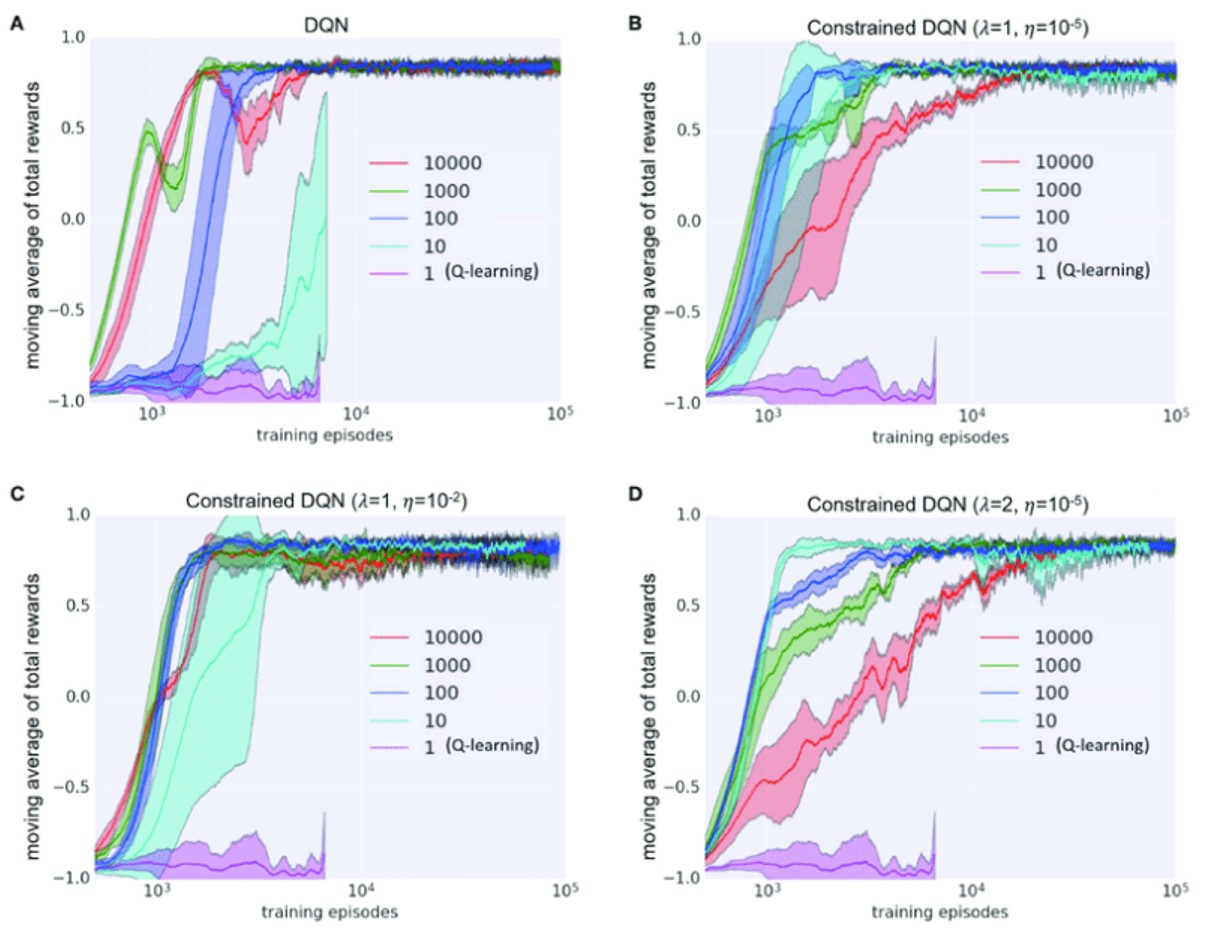
\includegraphics[width=0.7\textwidth]{3/figures/batch.jpg}
			\caption[Efectos de la frecuencia de actualización de la red objetivo en la tarea del laberinto MNIST]{Efectos de la frecuencia de actualización de la red objetivo en la tarea del laberinto MNIST\\
				Fuente: \citep*{gl_constr}. \citetitle{gl_constr}.}
			\label{1:fig}
		\end{center}
	\end{figure}
	\medskip
\end{itemize}
\textbf{Entregable:} Modelo DQN entrenado con una política optimizada de mapeo de estado del entorno a la acción que maximiza la recompensa esperada.

\end{itemize}
\item[c.] Planificar Ruta \\
Tomando en cuenta el entrenamiento del modelo DQN y la política optimizada, el agente utiliza dicha política desde el punto de origen para decidir el siguiente nodo en la ruta. Para esto, se utiliza una propagación hacia delante, donde cada paso que realiza el agente consulta a la política para saber si la acción minimiza el riesgo de crimen, asegurando que siempre se elija la mejor opción. Luego este proceso se realiza iterativamente hasta que el agente alcance el destino, construyendo una ruta completa y coherente. Además, se registra los índices de riesgo de cada nodo o arista seleccionada por el agente y se representa matemáticamente de la siguiente manera:
\begin{equation} 
	R_{total}=\sum_{i=1}^{N}r_{i}
\end{equation}
Donde $r_{i}$ es la probabilidad de riesgo de cada nodo o arista $i$, lo que proporciona una medida cuantitativa del riesgo para evaluar la efectividad del modelo.

\textbf{Entregable:} Subgrafo de la ruta resultante y el índice total de riesgo.

\end{itemize}

\subsection{Metodología para la medición de resultados}
\subsubsection{Evaluación del Modelo}
\begin{itemize}
	\item Root Mean Squared Error (RMSE)
	
	Se utiliza el RMSE para medir la precisión del modelo DGN propuesto en cuanto a las probabilidades de riesgo, cuantificando la desviación de las probabilidades de riesgo de cada nodo. Para esto, se utiliza la fórmula tradicional que es la siguiente:
	
\begin{equation} 
	RMSE = \sqrt{\frac{1}{N}\sum_{i=1}^{N}(y_{i}-\hat{y}_{i})^{2}}
\end{equation}
	
Donde:

$N$ es el total de nodos del grafo.

$y_{i}$ es la probabilidad de riesgo objetivo para nodo $i$.
	
$\hat{y}_{i}$ es la probabilidad de riesgo predicha por el modelo DGN para nodo $i$.
	
	Si el valor es bajo, quiere decir que las estimaciones de riesgo son precisas y asegura que el modelo propuesto es efectivo para la identificación de zonas de alto riesgo para que el agente pueda evitar dichas zonas en el proceso de entrenamiento DQN.
	
\textbf{Entregable:} Índice de efectividad del modelo DGN.
	\item Indicador de Riesgo \\
	Se utiliza la función de riesgo total establecido para la planificación de la ruta, y se evalúa el riesgo a cada ruta propuesta. Asimismo se establece un umbral que servirá de comparación con el riesgo total de una ruta, el cual determinará si la ruta se acepta o no. A continuación, se presenta el flujo condicional para la aceptación de la ruta:
	
	\begin{figure}[h]
		\begin{center}
			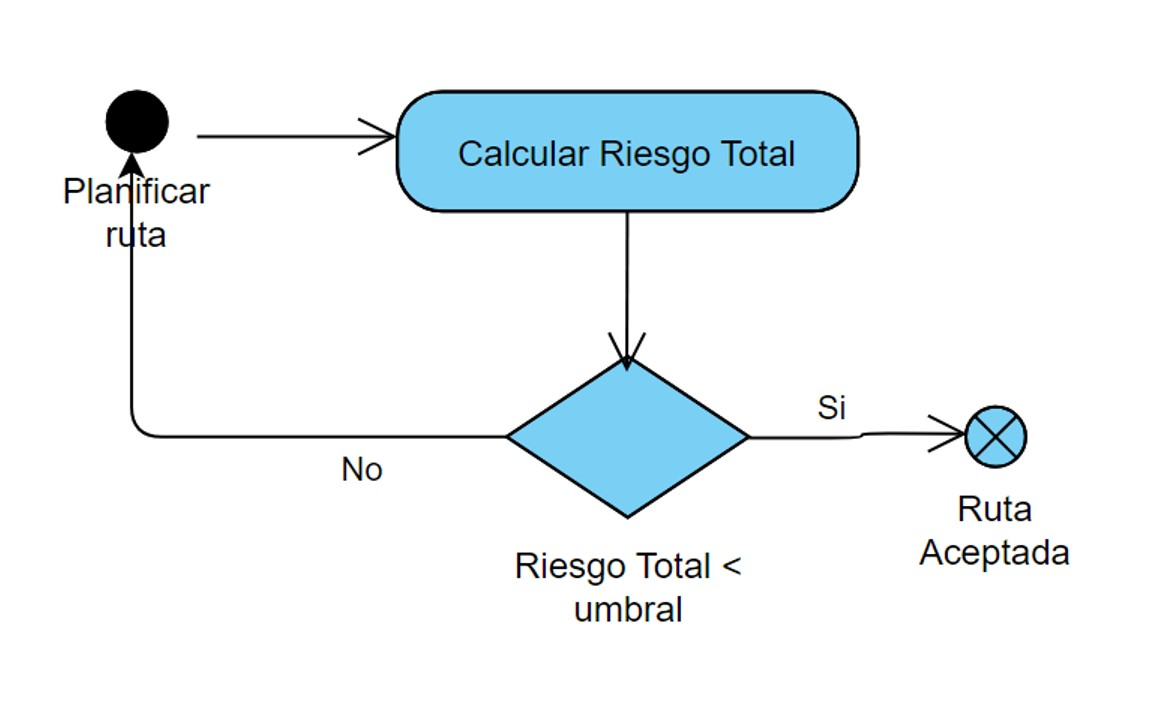
\includegraphics[width=0.65\textwidth]{3/figures/flujoCONDI.jpg}
			\caption[Elaboración propia: Flujo de condición de elección de ruta]{Elaboración propia: Flujo de condición de elección de ruta}
			\label{1:fig}
		\end{center}
	\end{figure}
	
\textbf{Entregable:} Ruta Segura con el menor índice de riesgo aceptada.
	\item Indicador de Eficiencia (TTM) \\
El indicador de Eficiencia (TTM) evalúa el rendimiento del modelo DRL, con el fin de proporcionar una medida cuantitativa para el tiempo de procesamiento del modelo y que se determina de la siguiente manera:
\begin{equation} 
	TTM = N_{ep} \times T_{ep}
\end{equation}

Donde: 

$N_{ep}$ es el número de épocas del modelo.

$T_{ep}$ el tiempo promedio necesario para completar una época en el entrenamiento.

Asimismo, se evalúa otro indicador de Eficiencia (TTM) que es para determinar el tiempo promedio de la ruta seleccionada, y puede ser representada de la siguiente manera:
\begin{equation} 
	TTM = \frac{Distancia \:de \:la\: ruta}{Velocidad \: Promedio}
\end{equation}
\textbf{Entregable:} Indicador de eficiencia del modelo DRL y de la ruta seleccionada.
\end{itemize}
\subsubsection{Visualización de la ruta}
Debido a que se trabaja con datos geoespaciales y el empleo de un modelo de planificación de rutas seguras, se propone utilizar la herramienta Folium en Python, ya que permite crear mapas interactivos que pueden ser explorados desde un navegador web, asimismo, se integra fácilmente con otras bibliotecas como Pandas, y personalizable. Esto es de ayuda para identificar patrones espaciales de riesgo y como la ruta seleccionada evita las zonas de alto riesgo.
	\begin{figure}[h]
	\begin{center}
		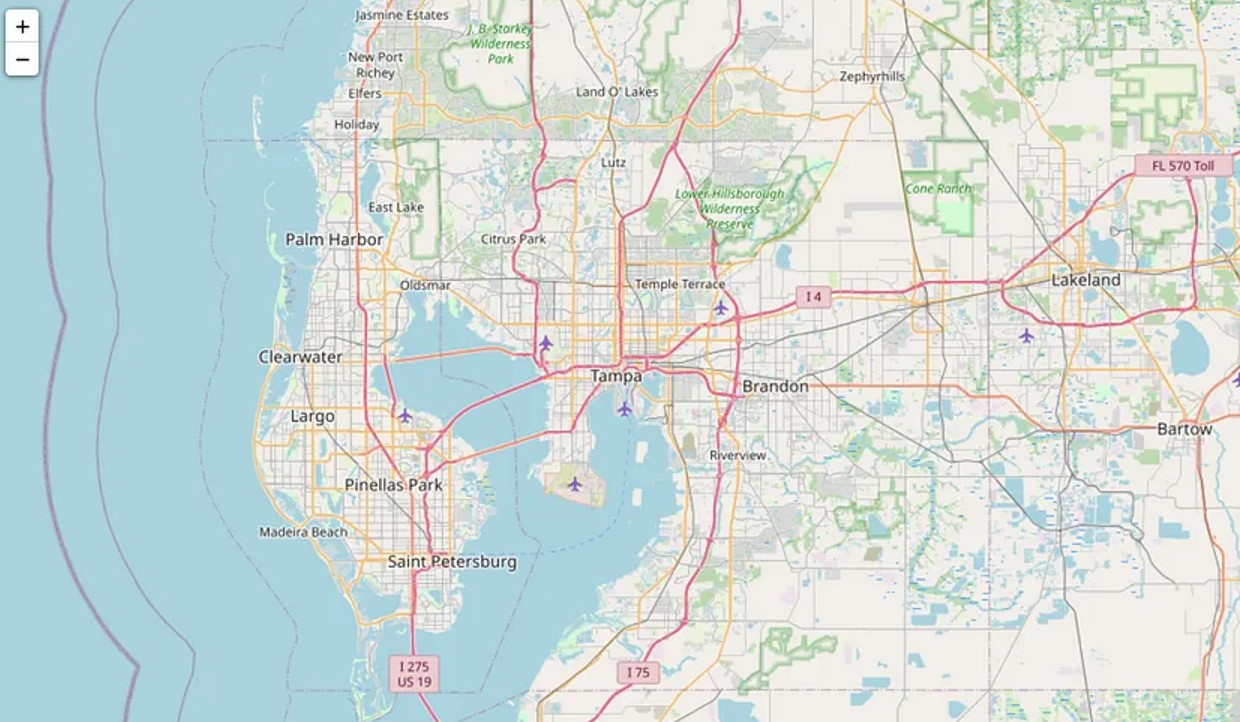
\includegraphics[width=0.65\textwidth]{3/figures/florida.jpg}
		\caption[Mapa de Tampa, Florida, creado en Folium y OpenStreetMap]{Mapa de Tampa, Florida, creado en Folium y OpenStreetMap\\
			Fuente: \citep*{gl_folium}. \citetitle{gl_folium}.}
		\label{1:fig}
	\end{center}
\end{figure}
\textbf{Entregable:} Visualización de la ruta segura seleccionada.

\begin{landscape}
	\section{Cronograma de actividades y presupuesto}
	Se elaboró un cronograma de actividades de toda la investigación, mostrada en la Figura \ref{1:fig1}, contemplando desde el inicio del mes de abril 2024 hasta la sustentación del trabajo estimado para inicios de diciembre 2024.
	
	\begin{figure}[!ht]
		\begin{center}
			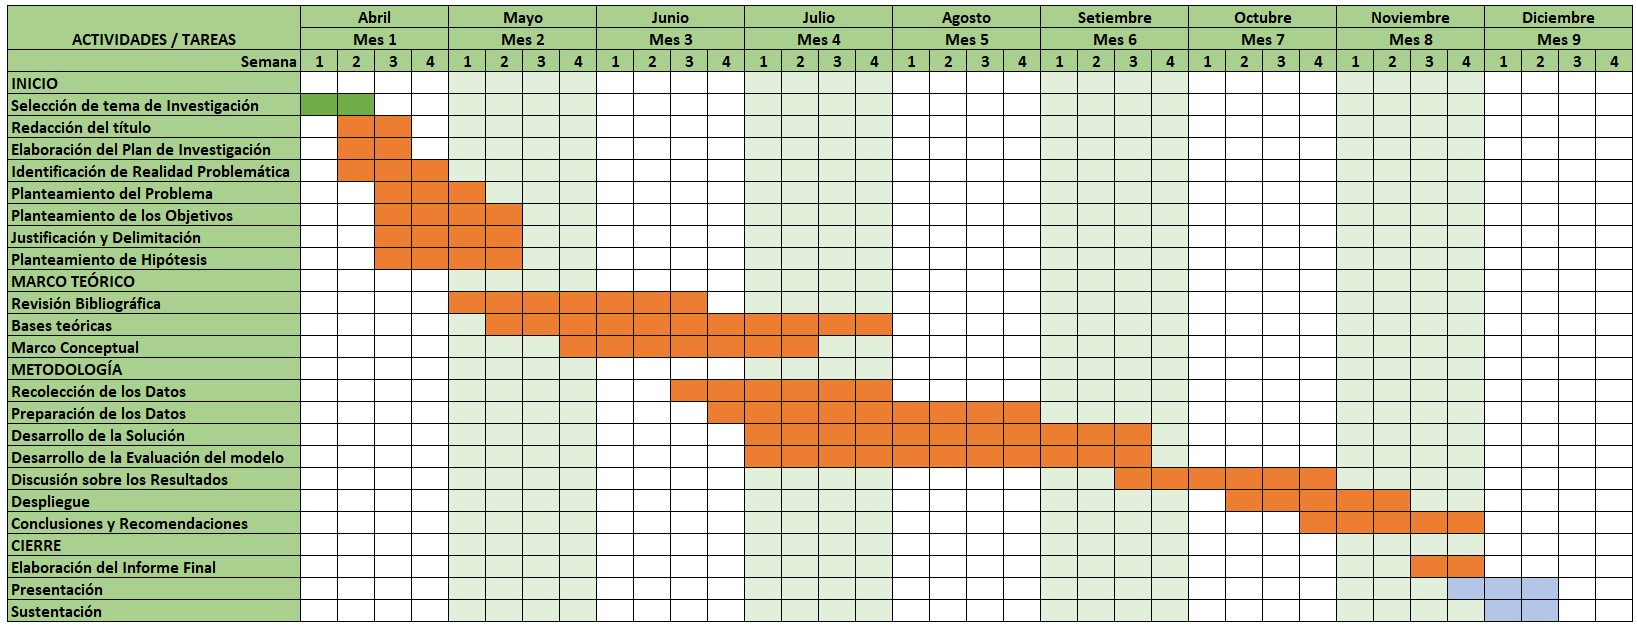
\includegraphics[width=1.55\textwidth]{3/figures/crono.jpg}
			\caption[Cronograma de actividades de la investigación]{Cronograma de actividades de la investigación.\\
				Fuente: Elaboración propia.}
			\label{1:fig1}
		\end{center}
	\end{figure}
	
\end{landscape}

A continuación, se muestra los costos personales del autor para la resolución del proyecto.

    \begin{table}[h!]
	\caption[Presupuesto de los costos personales del autor]{Presupuesto de los costos personales del autor.}
	\label{1:table}
	\centering
	\small
	\begin{tabular}{lcrr}
		\specialrule{.1em}{.05em}{.05em}
		\multicolumn{1}{c}{\centering{Item}} & \multicolumn{1}{c}{\centering{Tiempo usado (horas)}} & \multicolumn{1}{c}{\centering{Costo (soles)}} & \multicolumn{1}{c}{\centering{Subtotal}}
		\\
		\specialrule{.1em}{.05em}{.05em}
		\multicolumn{4}{l}{Recursos materiales}
		\\
		Laptop HP Pavilion Gaming Laptop 15 core i7 9750h 16GB  &  & S/.3,208.50 & S/.3,208.50
		\\
		\hline
		\multicolumn{4}{l}{Servicios generales}
		\\
		Internet + luz (9 meses) & \multicolumn{1}{r}{110} & S/.327.00 & S/.2,943.00
		\\
		\specialrule{.1em}{.05em}{.05em}
		Total &  &  & \multicolumn{1}{l}{S/.6,151.50}
		\\
		\specialrule{.1em}{.05em}{.05em}
	\end{tabular}
	\begin{flushleft}
		\small Fuente: Elaboración propia.
	\end{flushleft}
\end{table}
%\begin{table}[h]
%	\centering
%	\begin{tabular}{l|r}
%		Item & Quantity \\\hline
%		Widgets & 42 \\
%		Gadgets & 13
%	\end{tabular}
%	\caption{\label{tab:widgets}An example table.}
%\end{table}